\chapter{Письменность}
\section{Тибетский алфавит и его графемы}
Тибетские национальные грамматики делят тибетские графемы\prfnote{Графема --- минимальная единица письменности: в алфавитных системах письма --- буква (или другое отражение фонемы), в неалфавитных системах письма --- слоговой знак, иероглиф, идеограмма и другие.} на две категории: \prfC{གསལ་བྱེད་}{сэльце}{(букв. <<объясняющие, делающие ясным>>)} --- корневые, или основные, графемы и \prfC{དབྱངས་}{янг}{(букв. <<звучные>>)} --- некорневые графемы, или графемы-диакритики\footnote[9]{Все европейские грамматики тибетского языка называют первые графемы <<согласными буквами>>, а вторые --- <<гласными буквами>>. Такая терминология, по нашему мнению, неточна. Вернее было бы тибетские графемы противопоставлять по линии <<корневые (основные) --- некорневые (вспомогательные)>>, что отражает их действительные различия на уровне графики. Термины же <<согласные буквы>> и <<гласные буквы>> отражают различие тибетских графем лишь в фонетическом плане, не указывая при этом на их графическую неоднородность. Однако в отдельных случаях, когда необходимо отразить фонетическую значимость графем, мы будем пользоваться и терминами <<согласная>> и <<гласная>>, имея в виду соответственно корневые и некорневые графемы.}.

\emph{Корневые графемы} составляют тибетский алфавит, насчитывающий 30 знаков. Каждая корневая графема тибетского языка, за исключением графем \prfA{འ} и \prfA{ཨ} (см. таб. \ref{tab:1}), записывает слог, состоящий из двух элементов (звуков): согласного и присущего гласного \emph{a}, который на письме не обозначается. Каждому слогу присущ тон: либо ровный высокого регистра (\toneR), либо восходящий (\toneV). Кроме этих двух основных тонов можно выделить два дополнительных тона: восходяще-падающий (\toneVN) и падающий (\toneN), которые возникают при произношении двух корневых графем, когда одна приписывается к другой (см. \hyperref[sec:gss]{<<Графическая структура слога и его произношение>>}).

Все корневые графемы тибетского алфавита располагаются в определённом порядке: слева направо по классам и сверху вниз по рядам (см. таб. \ref{tab:1})\prfnote{Здесь и далее до описания систем транслитерации используется Международный фонетический алфавит \href{https://ru.wikipedia.org/wiki/Международный\_фонетический\_алфавит}{https://ru.wikipedia.org/wiki/Международный\_фонетический\_алфавит}. }.

\begin{tabularx}{\linewidth}{*{5}{c@{\hspace{2em}}}}
	\caption{Корневые графемы тибетского языка}\label{tab:1}
	\\
    \toprule
    \multirow{2}{*}{Класс} & \multicolumn{4}{c}{Ряд}\\
    \cmidrule{2-5}
	 & 1 & 2 & 3 & 4\\
	\endhead
	\midrule
	1 & \prfB{ཀ}{\mfa{ka}} \toneR & \prfB{ཁ}{\mfa{k'a}} \toneR & \prfB{ག}{\mfa{k'a}} \toneV & \prfB{ང}{\mfa{ṅa}} \toneV \\
	2 & \prfB{ཅ}{\mfa{tsja}} \toneR & \prfB{ཆ}{\mfa{ts'ja}} \toneR & \prfB{ཇ}{\mfa{ts'ja}} \toneV & \prfB{ཉ}{\mfa{nja}} \toneV \\
	3 & \prfB{ཏ}{\mfa{ta}} \toneR & \prfB{ཐ}{\mfa{t'a}} \toneR & \prfB{ད}{\mfa{t'a}} \toneV & \prfB{ན}{\mfa{na}} \toneV \\
	4 & \prfB{པ}{\mfa{pa}} \toneR & \prfB{ཕ}{\mfa{p'a}} \toneR & \prfB{བ}{\mfa{p'a}} \toneV & \prfB{མ}{\mfa{ma}} \toneV \\
	5 & \prfB{ཙ}{\mfa{tsa}} \toneR & \prfB{ཚ}{\mfa{ts'a}} \toneR & \prfB{ཛ}{\mfa{ts'a}} \toneV & \prfB{ཝ}{\mfa{wa}} \toneV \\
	6 & \prfB{ཞ}{\mfa{sja}} \toneV & \prfB{ཟ}{\mfa{sa}} \toneV & \prfB{འ}{\mfa{a}} \toneV & \prfB{ཡ}{\mfa{ja}} \toneV \\
	7 & \prfB{ར}{\mfa{ra}} \toneV & \prfB{ལ}{\mfa{la}} \toneV & \prfB{ཤ}{\mfa{sja}} \toneR & \prfB{ས}{\mfa{sa}} \toneR \\
	8 & \prfB{ཧ}{\mfa{ha}} \toneR & \prfB{ཨ}{\mfa{a}} & & \\
	\bottomrule
\end{tabularx}

Тибетские национальные грамматики делят корневые графемы от \prfB{ཀ}{\mfa{ka}} до \prfB{ཧ}{\mfa{ha}} на пять категорий в зависимости от твердости (\prfA{དམ་པ་}) произношения, называя эти категории родовыми:

\begin{tabularx}{\textwidth}{p{0.45\textwidth} p{0.45\textwidth}}
    \toprule
    \parbox{0.45\textwidth}{\centering Родовая категория} & \parbox{0.45\textwidth}{\centering Согласные}\\
    \midrule
    Мужской род (\prfA{ཕོ་}) & \parbox[t]{\linewidth}{\prfA{ཀ}, \prfA{ཅ}, \prfA{ཏ}, \prfA{པ}, \prfA{ཙ}\\  (произносятся наиболее твёрдо)}\\
    \addlinespace
	Средний род (\prfA{མ་ནིང་}) & \prfA{ཁ}, \prfA{ཆ}, \prfA{ཐ}, \prfA{ཕ}, \prfA{ཚ}\\
    \addlinespace
	Женский род (\prfA{མོ་}) & \prfA{ག}, \prfA{ཇ}, \prfA{ད}, \prfA{བ}, \prfA{ཛ}, \prfA{ཝ}, \prfA{ཞ}, \prfA{ཟ}, \prfA{འ}, \prfA{ཡ}\\
    \addlinespace
	Совершенно женский род (\prfA{ཤིན་ཏུ་མོ་}) & \prfA{ཤ}, \prfA{ས}, \prfA{ང}, \prfA{ཉ}, \prfA{ན}, \prfA{མ}\\
    \addlinespace
    Нейтральный род (\prfA{མོ་གཤམ་}) & \parbox[t]{\linewidth}{\prfA{ར}, \prfA{ལ}, \prfA{ཧ}\\(произносятся наиболее\\неопределённо)}\\
    \bottomrule
\end{tabularx}

Приведённое выше деление согласных на соответствующие родовые категории связано с позицией корневых морфем в слоге (см. разд. \hyperref[sec:gss]{<<Графическая структура слога и его произношение>>}).

\emph{Некорневые графемы}, или \emph{графемы-диакритики}, представляют собой четыре огласовки: \prfB{ ི}{\mfa{(i)}}, \prfB{ ུ}{\mfa{(u)}}, \prfB{ ེ}{\mfa{(e)}}, \prfB{ ོ}{\mfa{(o)}}. Первая, третья и четвертая надписываются к корневой графеме, вторая --- подписывается к ней, при этом соответственно меняется качество гласного \mfa{(а)}, присущего корневой графеме, например: \prfB{ཀ}{\mfa{ka}} $\rightarrow$ \prfB{ཀི}{\mfa{ki}}, \prfB{ཀུ}{\mfa{ku}}, \prfB{ཀེ}{\mfa{ke}},\prfB{ཀོ}{\mfa{ko}}. Корневая графема может сочетаться только с одной некорневой графемой, обозначающей огласовку.

\section{Графическая структура слога и его произношение}
\label{sec:gss}

На письме различаются простой и производный слоги. Простой слог состоит только из одной корневой графемы.

К такой корневой графеме могут присоединяться другие графемы, в результате чего образуется производный слог, причём данная корневая графема становится главным элементом слога --- основой, а остальные графемы --- составляющими слога.

По тибетской традиции усложнение производного слога идет в следующем порядке:
\begin{description}
	\item \fbox{1} --- основа слога, в качестве которой может выступить любая из 30 корневых графем тибетского алфавита.
	\item \fbox{2} --- приписные графемы \prfA{(རྗེས་འཇུག་)}, в качестве которых могут выступать 10 следующих корневых графем: \prfA{ག}, \prfA{ང}, \prfA{ད}, \prfA{ན}, \prfA{མ}, \prfA{བ}, \prfA{འ}, \prfA{ར}, \prfA{ལ}, \prfA{ས}.
	\item \fbox{3} --- вторичная приписная графема \prfA{(ཡང་འཇུག་)}, в качестве которой выступает корневая графема \prfA{ས}.
	\item \fbox{4} --- графемы-диакритики \prfA{ ི}, \prfA{ ུ}, \prfA{ ེ}, \prfA{ ོ}.
	\item \fbox{5} --- подписные графемы \prfA{(འདོགས་ཅན་)}, в качестве которых выступают корневые графемы \prfA{ཝ}, \prfA{ཡ}, \prfA{ར}, \prfA{ལ}.
	\item \fbox{6} --- префиксальные графемы \prfA{(སྔོན་ཨཇུག་)}, в качестве которых выступают корневые графемы \prfA{ག}, \prfA{ད}, \prfA{བ}, \prfA{མ}, \prfA{འ}.
	\item \fbox{7} --- надписные графемы \prfA{(མགོ་ཅན་)}, в качестве которых выступают корневые графемы \prfA{ར}, \prfA{ལ}, \prfA{ས}.
\end{description}

Таким образом, из 30 корневых графем в качестве составляющих элементов слога могут выступать только 12 корневых графем ( \prfA{ག}, \prfA{ང}, \prfA{ད}, \prfA{ན}, \prfA{བ}, \prfA{མ}, \prfA{ཝ}, \prfA{འ}, \prfA{ཡ}, \prfA{ར}, \prfA{ས}, \prfA{ལ} ) \footnote[10]{Одна и та же корневая графема может выступать в качестве разных составляющих элементов слога.}.

Из изложенного выше видно, что тибетский слог конструируется как по горизонтали (приписные и префиксальные графемы), так и по вертикали (графемы-диакритики, подписные и надписные графемы). Графически и схематически различные типы тибетских слогов от простого до самого сложного могут выглядеть следующим образом:

1) \prfA{ག་} $\rightarrow$ \fbox{1}; 2) \prfA{གངས་} $\rightarrow$ \fbox{1} \fbox{2} \fbox{3};
3) \prfA{གིང་} $\rightarrow$
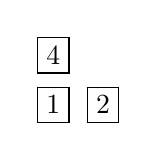
\begin{tikzpicture}[baseline=0pt]
	\draw (0pt,0pt) node {\fbox{1}};
	\draw (0pt,18pt) node {\fbox{4}};
	\draw (18pt,0pt) node {\fbox{2}};
\end{tikzpicture};
4) \prfA{གྲུབ་} $\rightarrow$
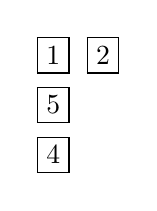
\begin{tikzpicture}[baseline=0pt]
	\draw (0pt,0pt) node {\fbox{1}};
	\draw (0pt,-18pt) node {\fbox{5}};
	\draw (0pt,-36pt) node {\fbox{4}};
	\draw (18pt,0pt) node {\fbox{2}};
\end{tikzpicture};

5) \prfA{སྒྲུབ་} $\rightarrow$
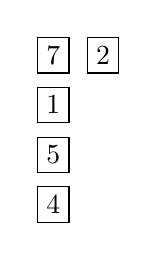
\begin{tikzpicture}[baseline=0pt]
	\draw (0pt,0pt) node {\fbox{7}};
	\draw (0pt,-18pt) node {\fbox{1}};
	\draw (0pt,-36pt) node {\fbox{5}};
	\draw (0pt,-54pt) node {\fbox{4}};
	\draw (18pt,0pt) node {\fbox{2}};
\end{tikzpicture};
6) \prfA{མགའ་} $\rightarrow$ \fbox{6} \fbox{1} \fbox{2};
7) \prfA{བསྐྲེངས་} $\rightarrow$
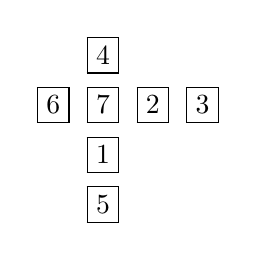
\begin{tikzpicture}[baseline=0pt]
	\draw (-18pt,0pt) node {\fbox{6}};
	\draw (0pt,18pt) node {\fbox{4}};
	\draw (0pt,0pt) node {\fbox{7}};
	\draw (0pt,-18pt) node {\fbox{1}};
	\draw (0pt,-36pt) node {\fbox{5}};
	\draw (18pt,0pt) node {\fbox{2}};
	\draw (36pt,0pt) node {\fbox{3}};
\end{tikzpicture};

Следует отметить, что тибетские корневые графемы пишутся по горизонтали в строчку. Над строчкой могут выступать только графемы-диакритики. В слогах, где имеются надписная и приписная графемы, основная графема опускается ниже строки, а приписная графема следует за надписной, как это видно из примеров 5 и 7.

Необходимо также отметить, что не каждая корневая графема, выступающая в качестве основы слога, может вступать в сочетание с любой подписной, надписной или приписной графемой. Некоторые же основы слога не могут вступать в сочетания и с целой группой составляющих слога. Так, например, корневые графемы \prfA{ཁ}, \prfA{ཆ}, \prfA{ཐ}, \prfA{ཕ}, \prfA{ཚ}, \prfA{ཝ}, \prfA{ཞ}, \prfA{ཟ}, \prfA{ཡ}, \prfA{ར}, \prfA{ལ}, \prfA{ས}, \prfA{ཨ}, \prfA{ཤ}, выступающие основой слога, не могут вступать в сочетания с надписными графемами. Корневые графемы \prfA{ཝ}, \prfA{འ}, \prfA{ར}, \prfA{ལ}, выступая основой слога, не могут принимать префиксальных графем и т.д.

Огласовки также не могут сочетаться с любой основой слога, особенно если последняя входит в состав производного слога. Это видно из следующей таблицы (таб. \ref{tab:2}). 

\begin{tabularx}{\textwidth}{p{0.1\textwidth} p{0.4\textwidth} p{0.4\textwidth}}
	\caption{Слоги, не принимающие огласовку}
	\label{tab:2}\\
		\toprule
	\parbox{0.1\textwidth}{\centering Огла\-совка} & \parbox{0.4\textwidth}{\centering Характер слога} & \parbox{0.4\textwidth}{\centering Слоги, не принимающие огласовку}\\
	\midrule
	\endhead
	\addlinespace
	\multirow[t]{4}{*}{\prfB{ ི}{\mfa{(i)}}} & простой & \prfA{ཁ}, \prfA{ང}, \prfA{ཕ}, \prfA{བ}, \prfA{ཝ}, \prfA{ཧ}\\
	& с надписными графемами & \prfA{རྐ}, \prfA{རྒ}, \prfA{རྔ}, \prfA{རྗ}, \prfA{རྣ}, \prfA{རྦ}|\quad  \prfA{ལྐ}, \prfA{ལྒ}, \prfA{ལྔ}, \prfA{ལྤ}, \prfA{ལྦ}, \prfA{ལྷ}|\quad \prfA{སྐ}, \prfA{སྒ}, \prfA{སྔ}, \prfA{སྣ}, \prfA{སྤ}, \prfA{སྦ}, \prfA{སྩ}\\
	\addlinespace
	& с подписными графемами & \prfA{མྱ}|\quad \prfA{ཏྲ}, \prfA{པྲ}|\quad \prfA{ཀླ}, \prfA{བླ}, \prfA{ཟླ}, \prfA{སླ}\\
	\addlinespace
	& с надписными и подписными графемами & \prfA{རྐྱ}, \prfA{རྒྱ}, \prfA{རྨྱ}|\quad \hl{??}\hyperref[tab:2:spec1]{$^*$},\prfA{རྩྭ}|\quad \prfA{ཕྱྭ}|\quad \prfA{གྲྭ},\prfA{སྨྲ}\\ 
	\midrule
	\addlinespace
	\multirow[t]{4}{*}{\prfB{ ུ}{\mfa{(u)}}} & простой & \prfA{ཝ}\\
	& с надписными графемами & \prfA{རྙ}, \prfA{རྦ}|\quad \prfA{ལྒ}, \prfA{ལྔ}, \prfA{ལྗ}, \prfA{ལྤ}|\quad \prfA{སྩ}\\
	\addlinespace
	& с подписными графемами & \prfA{པྱ}|\quad \prfA{ཏྲ}, \prfA{ཐྲ}, \prfA{པྲ}, \prfA{ཧྲ}\\
	\addlinespace
	& с надписными и подписными графемами & \prfA{རྐྱ}, \prfA{རྨྱ}|\quad \hl{??}\hyperref[tab:2:spec1]{$^*$}, \prfA{རྩྭ}|\quad \prfA{ཕྱྭ}|\quad \prfA{སྦྱ}|\quad \prfA{སྨྲ}\\
	\midrule
	\addlinespace
	\multirow[t]{4}{*}{\prfB{ ེ}{\mfa{(e)}}} & простой & \prfA{ཝ}, \prfA{འ}\\
	& с надписными графемами & \prfA{རྒ}, \prfA{རྣ}, \prfA{རྦ}|\quad \prfA{ལྐ}, \prfA{ལྒ}, \prfA{ལྔ}, \prfA{ལྗ}, \prfA{ལྤ}, \prfA{ལྦ}|\quad \prfA{སྔ}, \prfA{སྩ}\\
	\addlinespace
	& с подписными графемами & \prfA{པྱ}, \prfA{མྱ}|\quad \prfA{ཏྲ}, \prfA{ཐྲ}, \prfA{པྲ}|\quad \prfA{ཀླ}, \prfA{བླ}, \prfA{ཟླ}, \prfA{སླ}\\
	\addlinespace
	& с надписными и подписными графемами & \prfA{རྒྱ}, \prfA{རྨྱ}|\quad \hl{??}\hyperref[tab:2:spec1]{$^*$}, \prfA{རྩྭ}|\quad \prfA{ཕྱྭ}, \prfA{གྲྭ}|\quad \prfA{སྤྱ}, \prfA{སྦྱ}, \prfA{སྨྱ}\\
	\midrule
	\addlinespace
	\multirow[t]{4}{*}{\prfB{ ོ}{\mfa{(o)}}} & простой & \prfA{ཝ}\\
	& с надписными графемами & \prfA{ལྒ}, \prfA{ལྔ}, \prfA{ལྤ}, \prfA{ལྦ}\\
	\addlinespace
	& с подписными графемами & \prfA{དྲ}, \prfA{ཐྲ}, \prfA{མྲ}\\
	\addlinespace
	& с надписными и подписными графемами & \prfA{རྨྱ}|\quad \hl{??}\hyperref[tab:2:spec1]{$^*$}, \prfA{རྩྭ}|\quad \prfA{ཕྱྭ}|\quad \prfA{གྲྭ}|\quad \prfA{སྦྲ}\\
	\bottomrule
\end{tabularx}
{\footnotesize{\label{tab:2:spec1}* В таблице приведен слог, которые невозможно отобразить современными средствами: \textit{rgrwa}. Возможно, это описка. Следует уточнить в других источниках.}}
 
Производный слог с подписным \prfA{ཝ}, например: \prfA{ཀྭ}, \prfA{ཞྭ} и т.д., вообще не может иметь огласовок.

Тибетский производный слог читается по корневой графеме, выступающей основой слога. Компоненты производного слога оказывают влияние на чтение основы слога, определяя произношение слога в целом. Влияние компонентов слога может заключаться в: а) изменении тона корневой (читаемой) графемы; б) озвончении её; в) изменении качества гласного основы; г) появлении полугласного; д) изменении согласного звука основы; е) назализации согласного звука основы. Кроме этого, некоторые приписные графемы произносятся сами как конечный согласный слога или дают гортанную смычку. Некоторые префиксальные и надписные графемы не оказывают никакого влияния на звучание слога и играют только смыслоразличительную роль на письме. Все это наглядно иллюстрирует таб. \ref{tab:3}.

\begin{tabularx}{\textwidth}{X*{8}{c@{\hspace{1em}}}}
	\caption{Роли компонентов слога}
	\label{tab:3}\\
    \toprule
	\makecell[c]{Компонент слога} &
	\rotatebox{90}{\parbox{10em}{\small\raggedright Изменяет тон}} &
    \rotatebox{90}{\parbox{10em}{\small\raggedright Озвончает качество гласного}} &
    \rotatebox{90}{\parbox{10em}{\small\raggedright Изменяет качество гласного}} &
    \rotatebox{90}{\parbox{10em}{\small\raggedright Вводит полугласный}} &
    \rotatebox{90}{\parbox{10em}{\small\raggedright Изменяет согласный}} &
    \rotatebox{90}{\parbox{10em}{\small\raggedright Назализирует согласный}} &
    \rotatebox{90}{\parbox{10em}{\small\raggedright Читается как конечный согласный}} &
    \rotatebox{90}{\parbox{10em}{\small\raggedright Играет смыс\-ло\-раз\-ли\-чи\-тель\-ную роль на письме}}\\
	\midrule
	Приписные графемы & + & -- & + & -- & -- & -- & + & -- \\
	\addlinespace
	Подписные графемы & + & -- & -- & + & + & -- & -- & -- \\
	\addlinespace
	Префиксальные графемы & + & + & -- & -- & -- & + & -- & + \\
	\addlinespace
	Надписные графемы & + & + & -- & -- & -- & + & -- & + \\
	\bottomrule
\end{tabularx}
{\footnotesize{\emph{Примечание}. Знак + в таблице отнюдь не говорит, что вес компоненты слога данной группы (т.е. все приписные, все надписные и т.д.) играют в слоге указанную роль. Так, например, из 11 приписных только 4 меняют тон слога. Подробнее см. таб. \ref{tab:4}, \ref{tab:5}, \ref{tab:6}, \ref{tab:7}.}}

Каждая группа составляющих производного слога оказывает определённое влияние на его основу.

1.\emph{Приписные графемы} (за исключением \prfA{འ}\footnote[11]{\prfA{འ} служит для выделения основы слога в слоге, состоящем из двух корневых графем, не имеющих ни огласовки, ни подписного знака, например: в слоге \prfA{དགའ་} приписная \prfA{འ} указывает, что \prfA{ད} --- префиксальная графема, а \prfA{ག} --- основа; в слоге \prfA{དག་} отсутствие приписной \prfA{འ} указывает, что \prfA{ད} --- основа, а \prfA{ག} --- приписная. Сама приписная не оказывает влияния на звучание слога.}), входя в состав слога, оказывают то или иное влияние на его звучание. Приписная графема может: а) изменить ровный тон высокого регистра основы слога на падающий
( \toneR $\rightarrow$ \toneN ), восходящий тон на восходяще-падающий ( \toneV $\rightarrow$ \toneVN ); б) дать гортанную смычку ( \toneG ) удлинить или видоизменить гласный слога (см. таб. \ref{tab:4}).

2. \emph{Вторичная приписная графема}. За приписными \prfA{ག}, \prfA{ང}, \prfA{བ}, \prfA{མ} может следовать ещё одна приписная --- вторичная приписная графема --- \prfB{ས}{\mfa{sa}}. Если \prfA{ས} следует за приписными \prfA{ག} или \prfA{བ}, то она играет только смыслоразличительную роль на письме, например: \prfC{ཐབས་}{\mfa{t'ɘp}\toneN}{<<способ, метод>>} --- \prfC{ཐབ་}{\mfa{t'ɘp}\toneN}{<<печь, очаг>>}. Если же вторичная приписная следует за приписными \prfA{ང}, \prfA{མ}, то ровный тон слога меняется на падающий, а восходящий --- на восходяще-падающий, например: \prfC{ཐེང་}{\mfa{t'eŋ}\toneR}{<<хромой>>} ---  \prfC{ཐེངས་}{\mfa{t'eŋ}\toneN}{<<раз>>, <<один раз>>},\prfC{གང་}{\mfa{k'aŋ}\toneV}{<<где, куда>>} --- \prfC{གངས་}{\mfa{k'aŋ}\toneVN}{<<снег>>}.

\begin{tabularx}{\textwidth}{m{0.15\textwidth}m{0.5\textwidth}m{0.25\textwidth}}
	\caption{Приписные графемы}\label{tab:4}
	\\
	\toprule
	\makecell[c]{Приписная\\графема} & \makecell[c]{Её роль в слоге} & \makecell[c]{Примеры}\\
	\midrule
	\endhead
	\prfA{ག} & \makecell[c]{Меняет тон и\\ даёт гортанную смычку\\
$
\left.\begin{aligned}
\toneR \rightarrow \toneN \\
\toneV \rightarrow \toneVN \\
\end{aligned}\right\rbrace + 
$ \toneG } & \makecell{\prfB{ཐག་}{\mfa{t'a}}\toneG\toneN\\ \prfB{དག་}{\mfa{t'a}}\toneG\toneVN}\\
\addlinespace[1em]
\prfA{ས}, \prfA{ད} & \makecell[c]{Меняет тон и гласный основы\\ слога, даёт гортанную смычку\\
$
\left.\begin{aligned}
	\toneR \rightarrow \toneN \\
	\toneV \rightarrow \toneVN
\end{aligned}\right\rbrace + 
$ \makecell[l]{\mfa{a} $\rightarrow$ \mfa{ɛ} \\\mfa{u} $\rightarrow$ \mfa{y} + \toneG\\\mfa{o} $\rightarrow$ \mfa{ø}} }  & 
\makecell{
	\prfB{ཆས་}{\mfa{ts'ø}}\toneG\toneN\\
	\prfB{ཟས་}{\mfa{sɛ}}\toneG\toneVN\\
	\prfB{བོད་}{\mfa{p'ø}}\toneG\toneVN\\
	\prfB{ཕུད་}{\mfa{p'y}}\toneG\toneVN
}\\
\addlinespace[1em]
\prfA{བ} & \makecell[c]{Меняет тон и гласный \textit{a} основы \\слога, читается \textit{p}\\
$
\left.\begin{aligned}
	\toneR \rightarrow \toneN \\
	\toneV \rightarrow \toneVN
\end{aligned}\right\rbrace + p
$ \makecell[c]{\mfa{a} $\rightarrow$ \mfa{ɘ}}} &
\makecell{
	\prfB{ཁབ་}{\mfa{k'ɘp}}\toneN\\
	\prfB{གབ་}{\mfa{k'ɘp}}\toneVN
}\\	
\addlinespace[1em]
\prfA{ལ}, \prfA{འི}\hyperref[tab:4:spec1]{$^*$} & \makecell[c]{Меняет гласный основы \\слога и удлиняет его\\
$
\left.\begin{aligned}
	\toneR \rightarrow \toneN \\
	\toneV \rightarrow \toneVN
\end{aligned}\right\rbrace +
$ \makecell[l]{\mfa{a} $\rightarrow$ \mfa{ɛ:} \\\mfa{u} $\rightarrow$ \mfa{y:}\\\mfa{o} $\rightarrow$ \mfa{ø:}}} &
\makecell{
	\prfB{ཐལ་}{\mfa{t'ɛ:}}\toneR\\
	\prfB{ཁོལ་}{\mfa{k'ø:}}\\
	\prfB{སའི་}{\mfa{sɛ:}}\toneR\\
	\prfB{ཁོའི་}{\mfa{k'ø:}}\toneR
}\\	
\addlinespace[1em]
\prfA{ན} & \makecell[c]{Меняет гласный основы \\слога и читается как \mfa{ñ}\\
$
\left.\begin{aligned}
	\text{\mfa{a}} \rightarrow \text{\mfa{ɛ}} \\
	\text{\mfa{u}} \rightarrow \text{\mfa{y}} \\
	\text{\mfa{o}} \rightarrow \text{\mfa{ø}}\\
\end{aligned}\right\rbrace +
$ \mfa{ñ}} & 
\makecell{
	\prfB{ཕན་}{\mfa{p'ɛn}}\toneR\\
	\prfB{སོན་}{\mfa{søñ}}\toneR\\
	\prfB{གོན་}{\mfa{k'øñ}}\toneV\\
	\prfB{ཀུན་}{\mfa{kyñ}}\toneR
}\\	
\addlinespace[1em]
\prfA{ར} & \makecell[c]{Удлиняет гласный основы слога} & 
\makecell{
	\prfB{ཐུར་}{\mfa{tu:}}\toneR\\
	\prfB{མར་}{\mfa{ma:}}\toneV
}\\	
\addlinespace[1em]
\prfA{ང} & \makecell[c]{Читается как \mfa{ŋ}}&
\makecell{
	\prfA{གང་}{\mfa{k'aŋ}}\toneR\\
	\prfA{དང་}{\mfa{t'aŋ}}\toneV
}\\	
\addlinespace[1em]
\prfA{མ} & \makecell[c]{Читается как \mfa{m̃}} &
\makecell{\prfB{དམ་}{\mfa{t'am̃}}\toneV}\\	
\bottomrule
\end{tabularx}
{\footnotesize{\label{tab:4:spec1}*\prfA{འི} --- вариант притяжательной падежной частицы (см. \ref{04_06_ppch}), которая присоединятся к основе открытого слога, выступая как суффикс.}}

В древнеписьменном языке имелась ещё одна вторичная приписная --- \prfA{ད}, которая могла следовать за приписными \prfA{ན}, \prfA{ར}, \prfA{ལ}. Хотя эта приписная давно уже на письме не употребляется, однако до сего времени сохранилось её влияние на орфографию служебного слова, которое сочетается со словами, оканчивающимися на корневые графемы
\prfA{ན}, \prfA{ར}, \prfA{ལ} (см. разд.\hyperref[sec:ss]{<<Служебные слова>>}).

3. \emph{Префиксальные графемы}. Их наличие в слоге влияет на: а) тон и звонкость основы слога; б) звучание слога. Как влияют префиксальные графики на тон и звонкость основы слога, показано в таб. \ref{tab:5}.
\begin{tabularx}{\textwidth}{*{7}{>{\centering\arraybackslash}m{0.12\textwidth}}}
	\caption{Префиксальные графемы}\label{tab:5}\\
	\toprule
	\multirow[m]{2}{0.12\textwidth}{Пре\-фикс} & \multicolumn{6}{c}{\parbox[m]{0.72\textwidth}{\centering Основы, с которыми сочетается префиксальная графема}}\\
	\cmidrule{2-7}
	& \multicolumn{3}{c}{\parbox[m]{.36\textwidth}{\centering Остаются без изменения}} & \parbox[m]{0.12\textwidth}{\centering О\-звон\-ча\-ют\-ся} & \multicolumn{2}{c}{\parbox[m]{0.24\textwidth}{\centering Восходящий тон меняют на ровный}}\\
	\midrule
	\endhead
	\prfA{ག} & \prfA{ཅ} \prfA{ཏ} \prfA{ཙ} & & \prfA{ཤ} \prfA{ས} \prfA{ཞ} \prfA{ཟ} & \prfA{ད} & \prfA{ཉ} \prfA{ན} & \prfA{ཡ}\\
	\addlinespace
	\prfA{ད} & \prfA{ཀ} \prfA{པ} & & & \prfA{ག} \prfA{བ} & \prfA{ང} \prfA{མ} & \\
	\addlinespace
	\prfA{བ} & \prfA{ཀ} \prfA{ཅ} \prfA{ཏ} \prfA{ཙ} & & \prfA{ཤ} \prfA{ས} \prfA{ཞ} \prfA{ཟ} & \prfA{ག} \prfA{ད} & & \\
	\addlinespace
	\prfA{མ} & & \prfA{ཁ} \prfA{ཆ} \prfA{ཐ} \prfA{ཚ} & & \prfA{ག} \prfA{ཇ} \prfA{ད} \prfA{ཛ} & \prfA{ང} \prfA{ཉ} \prfA{མ} & \\
	\addlinespace
	\prfA{འ} & & \prfA{ཁ} \prfA{ཆ} \prfA{ཐ} \prfA{ཕ} \prfA{ཚ} & & \prfA{ག} \prfA{ཇ} \prfA{ད} \prfA{བ} \prfA{ཛ} & & \\
	\bottomrule
\end{tabularx}

На звучание слога оказывают влияние префиксы \prfA{མ} и \prfA{འ}, а также префикс \prfA{ད}, если он стоит перед основой слога \prfA{བ}.

Префиксы \prfA{མ} и \prfA{འ} придают основе слога назализацию, соответственна: а) {\mfa{ŋ}} --- перед основой \prfA{ག}; б) {\mfa{ñ}} --- перед основами \prfA{ཇ}, \prfA{ད}, \prfA{ཛ} и производными слогами \prfA{གྱ}, \prfA{གྲ}, \prfA{བྲ}; в) {\mfa{m̃}} --- перед основой \prfA{བ}, например: \prfB{མགའ་}{\mfa{ŋka}}\toneV, \prfB{འབང་}{\mfa{m̃paŋ}}\toneV, \prfB{མཛའ་}{\mfa{ñtsa}}\toneV.

Префикс \prfA{ད} c основой слога \prfA{བ} даёт следующее звучание: а) если гласный слога {\mfa{а}}, то {\mfa{p'}} переходит в {\mfa{w}}, например: \prfB{དབའ་}{\mfa{wa}}\toneR, \prfB{དབང་}{\mfa{waŋ}}\toneR; б) если гласный основы не {\mfa{а}}, то согласный не произносится вообще, например: \prfB{དབེན་}{\mfa{eñ}}\toneR, \prfB{དབུལ་}{\mfa{ü:}}\toneR, \prfB{དབྱ་}{\mfa{ja}}\toneR, \prfB{དབྱི་}{\mfa{ji:}}\toneR.

4. \emph{Подписные графемы}. \prfA{ཝ}, \prfA{ཡ}, \prfA{ར}, \prfA{ལ}, подписываясь под основой слога, меняют свое начертание (кроме \prfA{ལ}), и оказывают определённое влияние на произношение слога (см. таб. \ref{tab:6}).

\begin{tabularx}{\textwidth}{p{0.1\textwidth}p{0.1\textwidth}p{0.25\textwidth}p{0.45\textwidth}}
	\caption{Подписные графемы}\label{tab:6}\\
	\toprule
	\parbox[t]{0.1\textwidth}{\small\centering Под\-пис\-ная гра\-фе\-ма} & \parbox[t]{0.1\textwidth}{\small\centering Ха\-рак\-тер на\-чер\-та\-ния} & \parbox[t]{0.25\textwidth}{\small\centering Какие сложные графемы * образует} & \parbox[t]{0.45\textwidth}{\small\centering Роль в слоге}\\
	\midrule
	\endhead
	\prfA{ཝ} & \prfA{ ྭ} & \prfA{ཀྭ} \prfA{ཁྭ} \prfA{གྭ} \prfA{ཅྭ} \prfA{ཉྭ} \prfA{ཏྭ} \prfA{དྭ} \prfA{ཙྭ} \prfA{ཚྭ} \prfA{ཞྭ} \prfA{ཟྭ} \prfA{རྭ} \prfA{ལྭ} \prfA{ཤྭ} \prfA{སྭ} \prfA{ཧྭ} \prfA{གྲྭ} & Играет только смыслоразличительную роль на письме, например:
	\prfC{ཤ་}{\mfa{sja}\toneR}{<<мясо>>} --- \prfC{ཤྭ་}{\mfa{sja}\toneR}{<<олень>>};
	\prfC{རྩ་}{\mfa{tsa}\toneR}{<<корень>>} --- \prfC{རྩྭ་}{\mfa{tsa}\toneR}{<<трава>>}\\
	\addlinespace
	\multirow[t]{3}{*}{\prfA{ཡ}} & \multirow[t]{3}{*}{\prfA{ ྱ}} & 1) \prfA{ཀྱ} \prfA{ཁྱ} \prfA{གྱ} & Читается как \mfa{j}, например: \prfB{ཀྱ}{\mfa{kja}\toneR}, \prfB{ཁྱ}{\mfa{k'ja}\toneR}, \prfB{གྱ}{\mfa{k'ja}\toneV}\\
	& & 2) \prfA{པྱ} \prfA{ཕྱ} \prfA{བྱ} & Меняет чтение основы на \mfa{tsj} и \mfa{ts'j}, например: \prfB{པྱ}{\mfa{tsja}\toneR}, \prfB{ཕྱ}{\mfa{ts'ja}\toneR}, \prfB{བྱ}{\mfa{ts'ja}\toneR}\\
	& & 3) \prfA{མྱ} & Меняет чтение основы на \mfa{nj}, например: \prfB{མྱ}{\mfa{nja}\toneR}\\
	\addlinespace
	\multirow[t]{3}{*}{\prfA{ར}} & \multirow[t]{3}{*}{\prfA{ ྲ}} & 1) \prfA{ཀྲ} \prfA{ཏྲ}* \prfA{པྲ} \prfA{ཁྲ} \prfA{གྲ} \prfA{དྲ} \prfA{ཐྲ}* \prfA{ཕྲ} \prfA{བྲ} & Меняет чтение основы на \mfa{tš} и \mfa{tš'}, например: \prfA{ཀྲ} \prfA{ཏྲ} \prfA{པྲ} читаются \mfa{tša}\toneR; \prfA{ཁྲ} \prfA{ཐྲ} \prfA{ཕྲ} читаются \mfa{tš'a}\toneR; \prfA{གྲ} \prfA{དྲ} \prfA{བྲ} читаются \mfa{tša}\toneV\\
	& & 2) \prfA{ཧྲ} & Меняет чтение основы на \mfa{š}, например \prfB{ཧྲ}{\mfa{ša}}\toneR\\
	& & 3) \prfA{ནྲ} \prfA{མྲ} \prfA{ཤྲ} \prfA{སྲ} & Играет только смыслоразличительную роль на письме\\
	\addlinespace
	\multirow[t]{2}{*}{\prfA{ལ}} & \multirow[t]{2}{*}{\prfA{ ླ}} & 1) \prfA{ཀླ} \prfA{གླ} \prfA{བླ} \prfA{རླ} \prfA{སླ} & У \prfA{ག} \prfA{བ} \prfA{ར} меняет восходящий тон на ровный высокого регистра, а также меняет чтение основы на \mfa{la}, например: \prfB{ཀླ}{\mfa{la}}, \prfB{གླ}{\mfa{la}}\toneR\\
	& & 2) \prfA{ཟླ} & Меняет чтение основы на \mfa{da}, например: \prfB{ཟླ}{\mfa{da}}\\
	\bottomrule
\end{tabularx}
{\footnotesize * Сложные графемы, помеченные звёздочкой, употреблялись только в древнетибетском.}

5. \emph{Надписные графемы}. Их роль видна из следующей таблицы (таб. \ref{tab:7}).

\begin{tabularx}{\textwidth}{p{0.1\textwidth}p{0.1\textwidth}p{0.25\textwidth}p{0.45\textwidth}}
	\caption{Надписные графемы}\label{tab:7}\\
	\toprule
	\parbox[t]{0.1\textwidth}{\small\centering Над\-пис\-ная графема*} & \parbox[t]{0.1\textwidth}{\small\centering Характер начертания} & \parbox[t]{0.25\textwidth}{\small\centering Какие сложные графемы образует} & \parbox[t]{0.45\textwidth}{\small\centering Роль в слоге}\\
	\midrule
	\endhead
	\multirow[t]{3}{*}{\prfA{ར}} & \multirow[t]{3}{*}{\prfA{ར}} & 1) \prfA{རྐ} \prfA{རྟ} \prfA{རྩ} & Играет только смыслоразличительную роль на письме\\
	& & 2) \prfA{རྒ} \prfA{རྗ} \prfA{རྡ} \prfA{རྦ} \prfA{རྫ} & Озвончает основу, например: \prfB{རྒ}{\mfa{ka}\toneV}, \prfB{རྡ}{\mfa{ta}\toneV}\\
	& & 3) \prfA{རྔ} \prfA{རྙ} \prfA{རྣ} \prfA{རྨ} & Меняет восходящий тон на ровный высокого регистра, например: \prfB{རྔ}{\mfa{ŋa}\toneR}\\
	\addlinespace
	\multirow[t]{4}{*}{\prfA{ལ}} & \multirow[t]{4}{*}{\prfA{ལ}} & 1) \prfA{ལྐ} \prfA{ལྕ} \prfA{ལྟ} \prfA{ལྤ} & Играет только смыслоразличительную роль на письме, например: \prfC{རྟ་}{\mfa{ta}\toneR}{<<лошадь>>} --- \prfC{ལྟ་}{\mfa{ta}\toneR}{<<глядеть>>}\\
	& & 2) \prfA{ལྒ} \prfA{ལྗ} \prfA{ལྡ}, \prfA{ལྦ} & Озвончает и назализует основу, например: \prfB{ལྒ}{\mfa{ŋka}\toneV}; \prfB{ལྗ}{\mfa{ñsja}\toneV}; \prfB{ལྡ}{\mfa{ñsa}\toneV}; \prfB{ལྦ}{\mfa{m̃pa}\toneV}\\
	& & 3) \prfA{ལྔ} & Меняет восходящий тон на ровный высокого регистра, например: \prfB{ལྔ}{\mfa{ŋa}\toneR}\\
	& & 4) \prfA{ལྷ} & Меняет чтение, например: \prfB{ལྷ}{\mfa{lha}\toneR}\\
	\addlinespace
	\multirow[t]{3}{*}{\prfA{ས}} & \multirow[t]{3}{*}{\prfA{ས}} & 1) \prfA{སྐ} \prfA{སྟ} \prfA{སྤ} \prfA{སྩ} & Играет только смыслоразличительную роль на письме, например: \prfC{རྐང་}{\mfa{kaŋ}}{<<костный мозг>>} --- \prfC{སྐང་}{\mfa{kaŋ}}{<<наполнить, удовлетворять>>}\\
	& & 2) \prfA{སྒ} \prfA{སྡ} \prfA{སྦ} & Озвончает основу, например: \prfB{སྒ}{\mfa{ka}\toneV}, \prfB{སྡ}{\mfa{ta}\toneV}\\
	& & 3) \prfA{སྔ} \prfA{སྙ} \prfA{སྣ}, \prfA{སྨ} & Меняет восходящий тон на ровный высокого регистра, например: \prfB{སྔ}{\mfa{ŋa}\toneR}\\
	\bottomrule
\end{tabularx}
{\footnotesize{* Надписные графемы \prfA{ར} \prfA{ལ} \prfA{ས} помимо изменения тона играют также смысло различительную роль на письме, например \prfA{སྔ་} \prfA{ལྔ་} \prfA{རྔ་} звучат одинаково \mfa{ŋa}, но имеют различные значения --- соответственно: <<старый, прежний>>, <<пять>>, <<барабан>>; \prfA{སྙིང་} и \prfA{རྙིང་} читаются каждый \mfa{njiŋ}, но значат соответственно <<душа, сердце>> и <<старый, изношенный>>.}}

\section{Тон и звучание слогов в двусложном слове}

Приведённые выше правила чтения слогов полностью применимы только в отношении отдельного слога, т.е. когда слог выступает как самостоятельная лексическая или грамматическая единица. Подавляющее же большинство тибетских слов --- двусложные. В двусложных словах тоны и произношение слогов влияют друг на друга, в результате чего в них происходят изменения. Ниже приводятся наиболее характерные из этих изменений.

1. В двусложном слове изменяются тоны его составляющих (см. таб. \ref{tab:8}).

\begin{tabularx}{\textwidth}{ccc}
	\caption{Таблица смены тонов}\label{tab:8}\\
	\toprule
	\makecell{Тон\\первого\\слога} & \makecell{Тон\\второго\\слога} & \makecell{Тоны\\слогов\\в слове}\\ \midrule
	\endhead
	\toneR & \toneV & \toneR{} \toneR\\
	\toneR & \toneVN & \toneR{} \toneN\\
	\toneV & \toneV & \toneV{} \toneR\\
	\toneN & \toneR & \toneR{} \toneR\\
	\toneN & \toneN & \toneR{} \toneN\\
	\toneN & \toneVN & \toneR{} \toneN\\ \addlinespace
	\toneVN & \toneR & \toneV{} \toneR\\ \addlinespace
	\toneVN & \toneN & \toneV{} \toneN\\ \addlinespace
	\toneVN & \toneVN & \toneV{} \toneN\\ \addlinespace
	\bottomrule
\end{tabularx}

2. Согласные, которые записываются первыми пятью корневыми графемами третьего ряда тибетского алфавита (\prfA{ག}, \prfA{ཇ}, \prfA{ད}, \prfA{བ}, \prfA{ཛ}), выступая в качестве второго слога в слове, озвончаются, например: \prfB{ཡི}{\mfa{ji}\toneV} + \prfB{གེ}{\mfa{k'e}\toneV} $\rightarrow$ \prfC{ཡི་གེ་}{\mfa{ji}\toneV{}\mfa{ke}\toneR}{<<буква, письмена>>}.

3. В первом слоге слова приписная \prfA{ག} произносится \mfa{k}, например: \prfC{ངག་མ་}{\mfa{nak\toneV{}ma\toneR}}{<<речь>>}.

4. Если \prfB{བ}{\mfa{p'a}\toneV}, \prfB{བེ}{\mfa{p'e}\toneV} или \prfB{བོ}{\mfa{p'o}\toneV} являются вторым слогом двуслога, то \mfa{р'} переходит в \mfa{w}, например: \prfB{གཏའ་བ་}{\mfa{ta}\toneR{}\mfa{wa}\toneR}, \prfB{དཔའ་བོ་}{\mfa{pa}\toneR{}\mfa{wo}\toneR}, \prfB{པེ་བེ་}{\mfa{pe}\toneR{}\mfa{we}\toneR}, но \prfB{ནོན་བུ་}{\mfa{noñ}\toneV{}\mfa{p'y}\toneR}.

5. Если слоги слова содержат гласные звуки \mfa{i} и \mfa{a} или \mfa{y} и \mfa{a}, то в составе слова происходит трансформация: \mfa{a} + \mfa{i} $\rightarrow$ \mfa{ɘ} + \mfa{i}; \mfa{i} + \mfa{a} $\rightarrow$ \mfa{i} + \mfa{ɘ}; \mfa{у} + \mfa{a} $\rightarrow$ \mfa{у} + \mfa{ɘ}; \mfa{a} + \mfa{у} $\rightarrow$ \mfa{ɘ} + \mfa{у}, например: \prfB{ཟི་མ་}{\mfa{si\toneV{}mɘ\toneR}}, \prfB{མ་གི་}{\mfa{mɘ\toneV{}ki\toneR}}, \prfB{ཁ་ཆུ་}{\mfa{k'ɘ\toneR{}ts'u\toneR}}.

6. Если приписная первого слога \prfA{ང}, \prfA{ར} или \prfA{ལ}, а вторым слогом являются \prfA{བ} или \prfA{པ}, то вместо \mfa{wa} или \mfa{pa} соответственно произносят \mfa{ŋ}, \mfa{ra} или \mfa{la}. В этом случае приписные \prfA{ར} и \prfA{ལ}гласный не удлиняют, например:
\prfB{ཟོར་བ་}{\mfa{so}\toneV{}\mfa{ra}\toneR},
\prfB{ཡོལ་བ་}{\mfa{jö}\toneV{}\mfa{la}\toneR},
\prfB{ཡོང་བ་}{\mfa{joŋ}\toneV{}\mfa{ŋa}\toneR},
\prfB{ཐར་པ་}{\mfa{t'a}\toneR{}\mfa{ra}\toneR}.

7. Если слово построено путём удвоения слогов, то при наличии надписной или подписной корневая графема второго слога не произносится, а произносится надписная или подписная, например:
\prfB{ལྷོད་ལྷོད་}{\mfa{lhö}\toneR{}\mfa{lo}\toneR}, \prfB{ཧྲང་ཧྲང་}{\mfa{šaŋ}\toneR{}\mfa{raŋ}\toneR};
если надписных и подписных нет, а имеется приписная \prfA{བ} или \prfA{ག}, то во втором слоге она не произносится, например:
\prfB{ལེབ་ལེབ་}{\mfa{lep}\toneV{}\mfa{le}\toneN},
\prfB{ཞིབ་ཞིབ་}{\mfa{sjip}\toneV{}\mfa{sji}\toneG{}\toneN},
\prfB{རྡོག་རྡོག་}{\mfa{tok}\toneV{}\mfa{to}\toneR}.

8. Если первый слог слова открытый, а второй слог начинается с префиксальных графем \prfA{བ}, \prfA{མ} или \prfA{འ}, то эти префиксальные становятся читаемыми и соответственно произносятся \mfa{р}, \mfa{m} и \mfa{n}, например:
\prfB{ཡ་མཚན་}{\mfa{jam}\toneV{}\mfa{ts'ɛn}\toneR},
\prfB{ལྔ་བརྒྱ་}{\mfa{ŋap}\toneR{}\mfa{kja}\toneR},
\prfB{མེ་འཁོར་}{\mfa{men}\toneV{}\mfa{k'o:}\toneR}.

9. Если первый слог слова открытый, а второй слог имеет надписную \prfA{ར}, то эта надписная становится читаемой, например: \prfB{རྡོ་རྗེ་}{\mfa{tor}\toneV{}\mfa{tse}\toneR}. По такому же правилу иногда произносятся слова с надписными \prfA{ལ} во втором слоге (но не \prfA{ས}).

\section{Транслитерация}

При издании текстов в европейских странах часто не представляется возможным воспроизвести эти тексты в традиционной графике из-за трудности и дороговизны набора. Вместе с тем нельзя давать эти тексты и в транскрипции, так как несовпадение графики тибетского слова с его звучанием, большое количество омонимов (но не омографов) сильно затрудняет перевод транскрипции обратно в графику. Так, например, \mfa{luŋ\toneR} означает и <<река>> (\prfA{ཀླུང་}) и <<ветер>> (\prfA{རླུང་}); \mfa{ka\toneR{}wa\toneR} означает и <<столб>> (\prfA{ཀ་བ་}) и <<густой>> (\prfA{སྐ་བ་}). Поэтому при издании тибетских текстов прибегают к транслитерации, т.е. к транскрибированию всех графем, входящих в состав слога. Такая запись обычно не передаёт действительного звучания производного слога, но позволяет свободно осуществлять обратный перевод его в традиционную графику.

Существует ряд способов записи тибетских корневых графем латинскими литерами, предложенных тибетологами различных стран.

Впервые такая запись была произведена в латино-тибетском словаре, составленном капуцинами Джузеппе да Асколи, Франческо Мария да Тоурс, Доменико да Фано в период 1708-1713 гг.\footnote[12]{К настоящему времени этот словарь не сохранился. Парижская национальная библиотека имеет рукопись с извлечениями из этого словаря, содержащую 2500 слов.}

Затем передача тибетских слов латинскими литерами была осуществлена капуцином А. Георги в его учебнике тибетского языка\footnote[13]{См.: A.Georgi, Alphabetum tangutanum sive tibetanum, Romae, 1762.}, составленном для нужд католических миссионеров.

Однако впервые способ записи тибетских графем латинскими литерами как систему предложил основатель тибетологии --- венгр Чома де Кёрёши в своей грамматике тибетского языка\footnote[14]{См.: A.Cs.Körös, A grammar of Tibetan Language, Calcutta, 1834.}.

Специально вопросу о транскрипции посвящена работа Т. Уайли, вышедшая в 1959 г.\footnote[15]{См.: T.Wylie, A standart System of Tibetan Transcription, Narvard, 1959.}, а в 1964 г. появилась работа Е.Рихтера <<Основы фонетики лхасского диалекта>>\footnote[16]{E.Richter, Grundlagen des phonetik des Lhasa dialektes, Berlin, 1964.}.

Существует около 30 систем записи тибетских корневых графем латинскими буквами, большинство из которых в значительной части совпадает друг с другом. Наиболее близки системы, предложенные Чома де Кёрёши и Т. Уайли. Наиболее удобна для транслитерации, пожалуй, система Т. Уайли, не содержащая диакритических знаков. Ниже приводится шесть систем записи корневых графем тибетского алфавита латинскими буквами (см. \ref{tab:9}).

\begin{tabularx}{\textwidth}{*{7}c}
	\caption{Системы транслитерации корневых графем}\label{tab:9}\\
	\toprule
	\parbox[m]{0.12\textwidth}{\small\centering Корневая графема} & \parbox[m]{0.12\textwidth}{\small\centering Чома де Кёрёши} & \parbox[m]{0.12\textwidth}{\small\centering Х.А.Ешке} & \parbox[m]{0.12\textwidth}{\small\centering С.Ч.Дас} & \parbox[m]{0.12\textwidth}{\small\centering Ж.Бако} & \parbox[m]{0.12\textwidth}{\small\centering Т.Уайли} & \parbox[m]{0.12\textwidth}{\small\centering Е.Рихтер}\\
	\midrule
	\endhead
	%1
	\prfA{ཀ} & \textit{ka} & \textit{ka} & \textit{ka} & \textit{ka} & \textit{ka} & \textit{ka}\\
	\prfA{ཁ} & \textit{kha} & \textit{k'a} & \textit{kha} & \textit{kha} & \textit{kha} & \textit{kha}\\
	\prfA{ག} & \textit{ga} & \textit{ga} & \textit{ga} & \textit{ga} & \textit{ga} & \textit{ga}\\
	\prfA{ང} & \textit{nga} & \textit{\.{n}a} & \textit{\^{n}a} & \textit{\.{n}a} & \textit{nga} & \textit{\.{n}a}\\
	%2
	\prfA{ཅ} & \textit{cha} & \textit{ca} & \textit{ca} & \textit{\u{c}a} & \textit{ca} & \textit{t\u{s}a}\\ 
	\prfA{ཆ} & \textit{chha} & \textit{cha} & \textit{cha} & \textit{\u{c}ha} & \textit{cha} & \textit{t\u{s}ha}\\ 
	\prfA{ཇ} & \textit{ja} & \textit{ja} & \textit{ja} & \textit{\u{j}a} & \textit{ja} & \textit{d\u{z}a}\\ 
	\prfA{ཉ} & \textit{nya} & \textit{nya} & \textit{\~{n}a} & \textit{\~{n}a} & \textit{nya} & \textit{\~{n}a}\\ 
	%3
	\prfA{ཏ} & \textit{ta} & \textit{ta} & \textit{ta} & \textit{ta} & \textit{ta} & \textit{ta}\\
	\prfA{ཐ} & \textit{tha} & \textit{t'a} & \textit{tha} & \textit{tha} & \textit{tha} & \textit{tha}\\
	\prfA{ད} & \textit{da} & \textit{da} & \textit{da} & \textit{da} & \textit{da} & \textit{da}\\
	\prfA{ན} & \textit{na} & \textit{na} & \textit{na} & \textit{na} & \textit{na} & \textit{na}\\
	%4
	\prfA{པ} & \textit{pa} & \textit{pa} & \textit{pa} & \textit{pa} & \textit{pa} & \textit{pa}\\
	\prfA{ཕ} & \textit{pha} & \textit{p'a} & \textit{pha} & \textit{pha} & \textit{pha} & \textit{pha}\\
	\prfA{བ} & \textit{ba} & \textit{ba} & \textit{ba} & \textit{ba} & \textit{ba} & \textit{ba}\\
	\prfA{མ} & \textit{ma} & \textit{ma} & \textit{ma} & \textit{ma} & \textit{ma} & \textit{ma}\\
	%5
	\prfA{ཙ} & \textit{tsa} & \textit{tsa} & \textit{tsa} & \textit{ca} & \textit{tsa} & \textit{tsa}\\
	\prfA{ཚ} & \textit{ts'ha} & \textit{ts'a} & \textit{tsha} & \textit{cha} & \textit{tsha} & \textit{tsha}\\ 
	\prfA{ཛ} & \textit{dsa} & \textit{dza} & \textit{dsa} & \textit{ja} & \textit{dza} & \textit{dza}\\ 
	\prfA{ཝ} & \textit{wa} & \textit{wa} & \textit{ua} & \textit{va} & \textit{wa} & \textit{wa}\\
	%6
	\prfA{ཞ} & \textit{zha} & \textit{\'{z}a} & \textit{sha} & \textit{\u{z}a} & \textit{zha} & \textit{\u{z}a}\\ 
	\prfA{ཟ} & \textit{za} & \textit{za} & \textit{za} & \textit{za} & \textit{za} & \textit{za}\\
	\prfA{འ} & \textit{ha} & \textit{'a} & \textit{ha} & \textit{'a} & \textit{'a} & \textit{'a}\\
	\prfA{ཡ} & \textit{ya} & \textit{ya} & \textit{ya} & \textit{ya} & \textit{ya} & \textit{ya}\\
	%7
	\prfA{ར} & \textit{ra} & \textit{ra} & \textit{ra} & \textit{ra} & \textit{ra} & \textit{ra}\\
	\prfA{ལ} & \textit{la} & \textit{la} & \textit{la} & \textit{la} & \textit{la} & \textit{la}\\
	\prfA{ལ} & \textit{la} & \textit{la} & \textit{la} & \textit{la} & \textit{la} & \textit{la}\\
	\prfA{ཤ} & \textit{sha} & \textit{sa} & \textit{ca} & \textit{sa} & \textit{sha} & \textit{sa}\\
	%8
	\prfA{ས} & \textit{sa} & \textit{sa} & \textit{sa} & \textit{sa} & \textit{sa} & \textit{sa}\\
	\prfA{ཧ} & \textit{ha} & \textit{ha} & \textit{ha} & \textit{ha} & \textit{ha} & \textit{ha}\\
	\prfA{ཨ} & \textit{a} & \textit{'a} & \textit{a} & \textit{a} & \textit{a} & \textit{a}\\
	\bottomrule
\end{tabularx}

При транслитерации тибетского слога запись производится в строчку слева направо.

Графемы --- составляющие слога (приписные, надписные и т.п.) передаются только согласной буквой.

Буквы, записывающие нечитаемые графемы, иногда подчёркиваются.

Если в слоге имеется подписная графема, то присущий гласный основы слога пишется после неё, например:

\prfA{སྒྲུབ་} ---
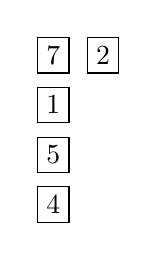
\begin{tikzpicture}[baseline=0pt]
	\draw (0pt,0pt) node {\fbox{7}};
	\draw (0pt,-18pt) node {\fbox{1}};
	\draw (0pt,-36pt) node {\fbox{5}};
	\draw (0pt,-54pt) node {\fbox{4}};
	\draw (18pt,0pt) node {\fbox{2}};
\end{tikzpicture}
$\rightarrow$ \textit{\ul{s}grub} -- \fbox{7} \fbox{1} \fbox{5} \fbox{4} \fbox{2}

\prfA{བསྐྲེངས་} ---
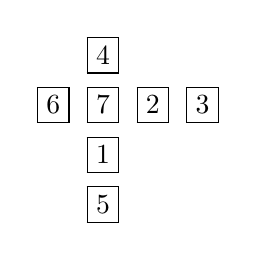
\begin{tikzpicture}[baseline=0pt]
	\draw (0pt,0pt) node {\fbox{6}};
	\draw (18pt,18pt) node {\fbox{4}};
	\draw (18pt,0pt) node {\fbox{7}};
	\draw (18pt,-18pt) node {\fbox{1}};
	\draw (18pt,-36pt) node {\fbox{5}};
	\draw (36pt,0pt) node {\fbox{2}};
	\draw (54pt,0pt) node {\fbox{3}};
\end{tikzpicture}
$\rightarrow$ \textit{\ul{bs}kreng\ul{s}} -- \fbox{6} \fbox{7} \fbox{1} \fbox{5} \fbox{4} \fbox{2} \fbox{3}

В последнее время предложены также различные системы транслитерации тибетских графем русскими буквами. Приводим одну из них: В.В. Семичова -- К. Седлачека (см. таб. \ref{tab:10}).

\begin{tabularx}{\textwidth}{*{8}c}
	\caption{Транслитерация русскими буквами}\label{tab:10}\\
	\toprule
	\parbox[m]{0.10\textwidth}{\small\centering Ти\-бет\-ские гра\-фе\-мы} & \parbox[m]{0.10\textwidth}{\small\centering Транс\-ли\-те\-ра\-ция} &
	\parbox[m]{0.10\textwidth}{\small\centering Ти\-бет\-ские гра\-фе\-мы} & \parbox[m]{0.10\textwidth}{\small\centering Транс\-ли\-те\-ра\-ция} &
	\parbox[m]{0.10\textwidth}{\small\centering Ти\-бет\-ские гра\-фе\-мы} & \parbox[m]{0.10\textwidth}{\small\centering Транс\-ли\-те\-ра\-ция} &
	\parbox[m]{0.10\textwidth}{\small\centering Ти\-бет\-ские гра\-фе\-мы} & \parbox[m]{0.10\textwidth}{\small\centering Транс\-ли\-те\-ра\-ция}\\
	\midrule
	\endhead
	\prfA{ཀ} & \textit{ка} & \prfA{ཁ} & \textit{кха} & \prfA{ག} & \textit{га} & \prfA{ང} & \textit{\.{н}а}\\
	\prfA{ཅ} & \textit{ча} & \prfA{ཆ} & \textit{чха} & \prfA{ཇ} & \textit{джа} & \prfA{ཉ} & \textit{ня}\\
	\prfA{ཏ} & \textit{та} & \prfA{ཐ} & \textit{тха} & \prfA{ད} & \textit{да} & \prfA{ན} & \textit{на}\\
	\prfA{པ} & \textit{па} & \prfA{ཕ} & \textit{пха} & \prfA{བ} & \textit{ба} & \prfA{མ} & \textit{ма} \\
	\prfA{ཙ} & \textit{ца} & \prfA{ཚ} & \textit{цха} & \prfA{ཛ} & \textit{дза} & \prfA{ཝ} & \textit{ва}\\
	\prfA{ཞ} & \textit{жа} & \prfA{ཟ} & \textit{за} & \prfA{འ} & \textit{'} & \prfA{ཡ} & \textit{я}\\
	\prfA{ར} & \textit{ра} & \prfA{ལ} & \textit{ла} & \prfA{ཤ} & \textit{ша} & \prfA{ས} & \textit{са}\\
	\prfA{ཧ} & \textit{ха} & \prfA{ཨ} & \textit{а} & & & & \\
	\bottomrule
\end{tabularx}

\section{Порядок расположения словарных статей в тибетско-тибетских и тибетско-европейских словарях}

Согласно тибетской лексикографической традиции, принятой и в тибетско-европейских словарях со времени выхода в свет <<Тибетско-русского словаря>> Я. Шмидта (СПб., 1843), все слова располагаются в алфавитном порядке корневых (читаемых) графем, а словарные статьи на одну корневую графему --- по степени усложнения производного слога.

Корневая графема выделяется по следующим формальным признакам:

1) графема, имеющая огласовку, надписную или подписную графему, является корневой. Так, например, в слоге \prfB{མཚོ་}{\ul{m}tsho}\footnote[17]{Здесь и ниже за тибетской графикой следует не транскрипция, а транслитерация по системе Т.Уайли (T. Wylie). Непроизносимые буквы подчёркиваются линейкой, слоги, входящие в состав одного слова, соединяются дефисами.} корневая графема --- \prfB{ཚ}{tsha}; в слоге \prfB{བསྡམ་}{\ul{bs}dam} корневая --- \prfB{ད}{da}; в слоге	\prfB{ངེས་}{nge\ul{s}} корневая - \prfB{ང}{nga}; в слоге \prfB{བསླད་}{\ul{bs}la\ul{d}} корневая --- \prfB{ས}{sa} (в данном случае \prfB{ལ}{la} не может быть корневой, поскольку к ней не надписывается \prfB{ས}{sa});

2)	если слог не имеет указанных выше компонентов, то: а) в слоге, состоящем из двух графем, первая будет корневой, например:
\prfB{ནང་}{nang} --- корневая \prfB{ན}{na};
\prfB{ཞག་}{zhag} --- корневая \prfB{ཞ}{zha};
\prfB{དག་}{dag} ---	корневая \prfB{ད}{da};
б) в слоге, состоящем из трёх графем, средняя --- корневая, например:
\prfB{དཔལ}{\ul{d}pa\ul{l}} --- корневая \prfB{པ}{pa};
\prfB{མནར་}{\ul{m}nar} --- корневая \prfB{ན}{na};
\prfB{གདས་}{\ul{g}da\ul{s}} --- корневая \prfB{ད}{da}.
Исключение из этого правила составляет случай, когда третьей графемой является \prfB{ས}{sa} следующая за графемами \prfB{ག}{ga}, \prfB{ང}{nga}, \prfB{བ}{ba} или \prfB{མ}{ma}. В этом случае \prfB{ས}{sa} выступает как вторичная приписная, а корневой будет первая графема, например:
\prfB{ཐགས་}{thag\ul{s}} --- корневая \prfB{ཐ}{tha};
\prfB{གངས་}{gang\ul{s}} --- корневая \prfB{ག}{ga};
\prfB{ཆབས་}{chab\ul{s}} --- корневая \prfB{ཆ}{cha};
\prfB{ཁམས་}{kham\ul{s}} --- корневая \prfB{ཁ}{kha}.

Усложнение слога, степенью которого определяется место того или иного слова в словаре, происходит в следующем порядке.

Слоги первой степени сложности представляют собой сочетания корневой графемы с приписной или с приписной в сочетании со вторичной приписной графемами. При этом место слова в словаре определяется алфавитным порядком приписной графемы по формуле:
\begin{equation*}
a(b_{1} + b_{1}c + b_{2} + b_{2}c + \dots{}b_{10}c)
\end{equation*}
где <<$a$>> --- корневая: <<$b_{1-10}$>> --- приписные и <<$c$>> — вторичная приписная.

Слоги второй степени сложности представляют собой сочетания корневой графемы с предыдущими компонентами и четырьмя огласовками по формуле:
\begin{equation*}
	a(d_{1} + d_{1}b_{1} + d_{1}b_{1}c + \dots{}d_{1}b_{10}c + d_{2} + d_{2}b_{1} + \dots{}\dots{}d_{4}b_{10}c)
\end{equation*}
где <<$d_{1-4}$>> --- четыре огласовки.

Слоги третей степени сложности представляют собой сочетания корневой с подписными графемами в алфавитном порядке, при этом каждая подписная графема последовательно сочетается с предыдущими компонентами.

Слоги четвертой степени сложности представляют собой сочетания корневой графемы с приписными в их алфавитном порядке.

Следующая и последняя степень сложности образуется сочетанием корневой с надписными графемами в их алфавитном порядке.
